\documentclass[a4paper]{article}
\usepackage[T1]{fontenc}
\usepackage[english]{babel}
\usepackage{clrscode4e} % Algorithm template from Introduction to Algorithms 4th
\usepackage[left=2cm,right=2cm,top=1cm,bottom=2cm]{geometry} % page settings
\usepackage{amsthm, amsmath, amssymb} % provides many mathematical environments & tools
\usepackage{tikz} % draw pictures
\usepackage{tabularray}
\usepackage[noend]{algorithmic}
\usepackage{tabularx}
\usepackage{algorithm}
\usepackage{arydshln}
\usepackage{forest}
% rotation
\usepackage{adjustbox}
\usepackage{array}
\usepackage{ifthen}
% figure caption
\usepackage{caption}
\usepackage{subfig}
\usepackage{graphicx,wrapfig,lipsum}
% arrays and matrices
\usepackage{nicematrix}
% line change inside cells
\usepackage{makecell}
%-----------------------------------------------------------
% Custom commands
%-----------------------------------------------------------
\newenvironment{hashtable}[1][]
  {\begin{tabular}[#1]{
     @{}
     > {\small} r <{\normalsize~\rlap{\fbox{\strut~~}}$~~\rightarrow$~}
     @{} l @{}}}
  {\end{tabular}}

\tikzset{
node of list/.style = {
             draw,
             fill=orange!20,
             minimum height=6mm,
             minimum width=6mm,
             node distance=6mm
   },
link/.style = {
     -stealth,
     shorten >=1pt
     },
array element/.style = {
    draw, fill=white,
    minimum width = 6mm,
    minimum height = 10mm
  }
}

\def\LinkedList#1{%
  \foreach \element in \list {
     \node[node of list, right = of aux, name=ele] {\element};
     \draw[link] (aux) -- (ele);
     \coordinate (aux) at (ele.east);
  }
}

\usetikzlibrary{positioning,matrix, arrows.meta}
\tikzset{box/.style={draw, thick, minimum width=1cm, minimum height=1cm}}

\newcommand{\Mod}[1]{\ (\mathrm{mod}\ #1)}

\newenvironment{solution}
  {\begin{proof}[Solution]}
  {\end{proof}}
\renewcommand{\qedsymbol}{\rule{0.7em}{0.7em}}

\makeatletter
\renewenvironment{proof}[1][\proofname]{%
  \par\pushQED{\qed}\normalfont%
  \topsep6\p@\@plus6\p@\relax
  \trivlist\item[\hskip\labelsep\bfseries#1\@addpunct{.}]%
  \ignorespaces
}{%
  \popQED\endtrivlist\@endpefalse
}
\makeatother
\setlength{\parindent}{0mm}

%-----------------------------------------------------------
% Document
%-----------------------------------------------------------
\begin{document}

\title{Algorithms: Homework 2}
\author{Li-Yuan Wei}
\date{\today}
\maketitle

\subsection*{Problem 1}
Using Figure 8.3 as a model, illustrate the operation of RADIX-SORT on the following list of English words: NOD, HOG, SHY, BAN, BAR, JET, EBB, PAR, ASH, PET, TED, ROT, FIG.
$$
\begin{array}{cccc}
0(initial)& digit\ 1 & digit\ 2 & digit\ 3 \\\\
\hline
\text{NOD} & \text{EB$\textbf{B}$} & \text{B$\textbf{A}$N} & \text{$\textbf{A}$SH} \\\\
\text{HOG} & \text{NO$\textbf{D}$} & \text{B$\textbf{A}$R} & \text{$\textbf{B}$AN} \\\\
\text{SHY} & \text{TE$\textbf{D}$} & \text{P$\textbf{A}$R} & \text{$\textbf{B}$AR} \\\\
\text{BAN} & \text{HO$\textbf{G}$} & \text{E$\textbf{B}$B} & \text{$\textbf{E}$BB} \\\\
\text{BAR} & \text{FI$\textbf{G}$} & \text{T$\textbf{E}$D} & \text{$\textbf{F}$IG} \\\\
\text{JET} & \text{AS$\textbf{H}$} & \text{J$\textbf{E}$T} & \text{$\textbf{H}$OG} \\\\
\text{EBB} & \text{BA$\textbf{N}$} & \text{P$\textbf{E}$T} & \text{$\textbf{J}$ET} \\\\
\text{PAR} & \text{BA$\textbf{R}$} & \text{S$\textbf{H}$Y} & \text{$\textbf{N}$OD} \\\\
\text{ASH} & \text{PA$\textbf{R}$} & \text{F$\textbf{I}$G} & \text{$\textbf{P}$AR} \\\\
\text{PET} & \text{JE$\textbf{T}$} & \text{N$\textbf{O}$D} & \text{$\textbf{P}$ET} \\\\
\text{TED} & \text{PE$\textbf{T}$} & \text{H$\textbf{O}$G} & \text{$\textbf{R}$OT} \\\\
\text{ROT} & \text{RO$\textbf{T}$} & \text{R$\textbf{O}$T} & \text{$\textbf{S}$HY} \\\\
\text{FIG} & \text{SH$\textbf{Y}$} & \text{A$\textbf{S}$H} & \text{$\textbf{T}$ED} \\\\
\end{array}
$$

\subsection*{Problem 2}
Show how to sort $n$ integers in the range $0$ to $n^2-1$ in $\mathcal{O}(n)$ time.
\begin{solution}
  Psuedocode for sorting $n$ integers in $\mathcal{O}(n)$, $X$ is an array storing all $n$ integers:\\
\noindent
\begin{tabularx}{\textwidth}{>{\footnotesize}rX@{}}
  \\[-1.5ex] \hline
  \multicolumn{2}{@{}l}{\refstepcounter{algorithm}\label{sort-n} $\proc{SORT-N-LINEAR}(X, n)$} \\
  \hline
   1: & \If $n == 1$ \\
   2: & \quad \Return \\
   3: & \For $i \gets 1$ \To $n$ \\
   4: & \quad \Comment change $X[i]$ into base $n$\\
   5: & \quad $\proc{TO-BASE-N}(X[i])$ \\
   6: & \Comment each integer will have at most $\log_n n^2 = 2$ digits\\
   7: & \Comment radix sort uses counting sort to sort $n$ at most $2$ digits integers\\
   8: & $\proc{RADIX-SORT}(X)$ \\
   9: & \For $i \gets 1$ \To $n$ \\
   10: & \quad \Comment convert $X[i]$ back to its original value because we sorted them with base $n$\\
   11: & \quad $\proc{CONVERT-BASE-N}(X[i])$ \\
\hline
\\ [-0.2cm]
\end{tabularx}

$\proc{TO-BASE-N}$ converts an integer into a base $n$ number. E.g. 100 integers have the largest number of 9999, which can be converted to base 100, $9999 = 99 * 100^1 + 99 * 100^0$. Originally, radix sort will sort 4 digits for 9999. After converting its base to $n$, radix sort will need to sort \textbf{2 digits} $99_{100}$ and $99_{100}$. Another example that the integer 400 will be converted to $4_{100}$. The \textbf{digit} here is not limit from 0 to 9.
\end{solution}

\subsection*{Problem 3}
Using Figure 8.4 as a model, illustrate the operation of BUCKET-SORT on the array $A$=<.49, .30, .56, .74, .68, .50, .69, .37, .41, .72>
\begin{figure}[H]
\centering
\begin{minipage}{5cm}
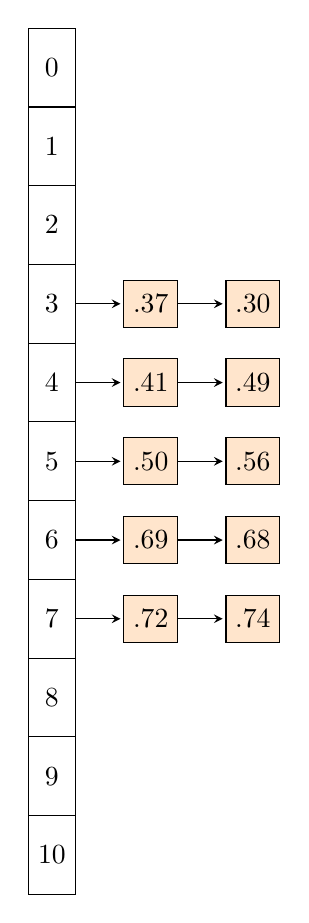
\begin{tikzpicture}
  \foreach \index/\list in {0/{}, 1/{}, 2/{}, 3/{.37,.30}, 4/{.41, .49}, 5/{.50, .56}, 6/{.69, .68}, 7/{.72, .74}, 8/{}, 9/{}, 10/{}} {
   \node[array element] (aux) at (0,-\index) {\index};
   \LinkedList{\list}
}
\end{tikzpicture}
\caption{Insert data}
\end{minipage}
\qquad
\begin{minipage}{5cm}
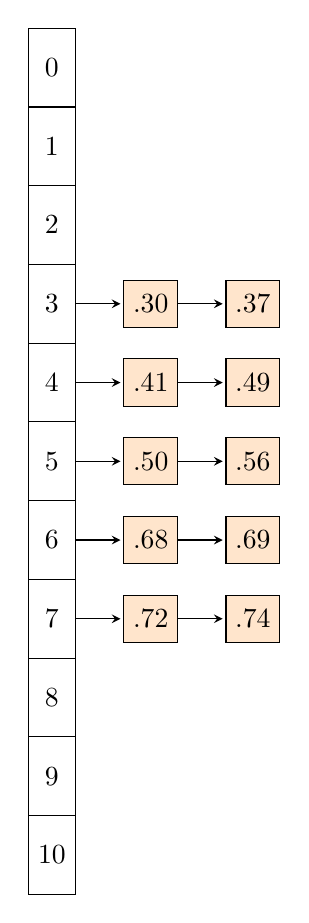
\begin{tikzpicture}
  \foreach \index/\list in {0/{}, 1/{}, 2/{}, 3/{.30,.37}, 4/{.41, .49}, 5/{.50, .56}, 6/{.68, .69}, 7/{.72, .74}, 8/{}, 9/{}, 10/{}} {
   \node[array element] (aux) at (0,-\index) {\index};
   \LinkedList{\list}
}
\end{tikzpicture}
\caption{Sort each bucket}
\label{bucket}
\end{minipage}
\end{figure}

\begin{solution}
To get sorted data, chain all the nodes in Figure \ref{bucket} from bucket $0$ to bucket $10$: \\
$<.30, .37, .41, .49, .50, .56, .68, .69, .72, .74>$
\end{solution}

\subsection*{Problem 4}
Suppose that you have a “black-box” worst-case linear time median subroutine. Give a simple, linear-time algorithm that solves the selection problem for an arbitrary order statistic.
\begin{solution}
  Psuedocode for finding the $k$-th smallest element in array $X[1..n]$, and assume $n > 0$:\\
\noindent
\begin{tabularx}{\textwidth}{>{\footnotesize}rX@{}}
  \\[-1.5ex] \hline
  \multicolumn{2}{@{}l}{\refstepcounter{algorithm}\label{find-k} $\proc{FIND-K-TH-SMALLEST}(X, n, k)$} \\
  \hline
  1: & $half = 0$ \\
  2: & \If n \% 2 == 1 \Comment n is odd\\
  3: & \quad $half = \lceil n / 2 \rceil$ \\
  4: & \textbf{else} \Comment n is even\\
  5: & \quad $half = n / 2$ \\
  6: & m = $\proc{BLACK-BOX}(X)$ \\
  7: & \If $k == half$ \Comment $k$-th smallest is median\\
  8: & \quad \Return $m$ \\
  9: & \Comment splits $X$ into two arrays, $Y$ contains elements less than $m$ and $Z$ contains elements greater than $m$\\
  10: & $Y, Z = \proc{SPLIT}(X, m)$\\
  11: & \If $k < half $ \\
  12: & \quad \Return $\proc{FIND-K-TH-SMALLEST}(Y, half, k)$\\
  13: & \textbf{else} \Comment $k > half$ \\
  14: & \quad \Comment Find $k - half$-th smallest for $Z$ since it's half the size of $X$\\
  15: & \quad \Return $\proc{FIND-K-TH-SMALLEST}(Z, half, k - half)$\\
\hline
\\ [-0.2cm]
\end{tabularx}

$T(n) = T(n/2) + \mathcal{O}(n)$($\proc{SPLIT}$). Apply master method $n^{\log_{b}a} = n^{\log_{2}1} = n^0 = 1 < \mathcal{O}(n)$, may apply case 3. First, we find $\epsilon = 1$ where $f(n) = \Omega(n^{(\log_{2}1) + \epsilon})$. Second, we find $c = 1/2$ where $af(n/b) = n/2 \le 1/2n = cf(n)$ is true. Thus, we can conclude that the running time of this algorithm is $\Theta(f(n)) = \Theta(n)$.
\end{solution}

\subsection*{Problem 5}
Let $X[1 .. n]$ and $Y[1 .. n]$ be two arrays, each containing $n$ numbers already in sorted order. Give an $\mathcal{O}(\lg n)$-time algorithm to find the median of all $2n$ elements in arrays $X$ and $Y$.
\begin{solution}
  Psuedocode for finding the median of arrays $X[1..n]$ and $Y[1..n]$, $xi$ is X array's starting index and $xj$ is X array's last index; $yi$ is $Y$ array's starting index and $yj$ is $Y$ array's last index:\\
\noindent
\begin{tabularx}{\textwidth}{>{\footnotesize}rX@{}}
  \\[-1.5ex] \hline
  \multicolumn{2}{@{}l}{\refstepcounter{algorithm}\label{find-median} $\proc{FIND-MEDIAN}(X,Y,xi,xj,yi,yj,n)$} \\
  \hline
   1: & \If $n == 1$\\
   2: & \quad \Comment Both arrays have only one element, pick the smaller one as median\\
   3: & \quad \Return $\proc{MIN}(X[1],Y[1])$\\
   4: & $xmid = X[(xi + xj) / 2]$ \Comment $X$'s median\\
   5: & $ymid = Y[(yi + yj) / 2]$ \Comment $Y$'s median \\
   6: & \If $xmid < ymid$ \\
   7: & \quad \Comment median must be greater than $xmid$ and less than $ymid$ \\
   8: & \quad \Return $\proc{FIND-MEDIAN}(X, Y, xmid + 1, xj, yi, ymid, n / 2)$\\
   9: & \textbf{else}\\
   10: & \quad \Comment median must be less than $xmid$ and greater than $ymid$ \\
   11: & \quad \Return $\proc{FIND-MEDIAN}(X, Y, xi, xmid, ymid + 1, yj, n / 2)$\\
\hline
\\ [-0.2cm]
\end{tabularx}
$T(n) = T(n/2) + \mathcal{O}(1)$ \\
Apply master method case 2 because $n^{\log_b{a}} = n^{\log_2{1}} = n^{0} = 1 = f(n)$. \\
$T(n) = \Theta({n^{\log_2{1}}\lg n}) = \Theta({\lg n})$.
\end{solution}

\subsection*{Problem 6}
Demonstrate the insertion of the keys 23, 38, 19, 40, 29, 43, 12, 27, 11 into a hash tale with collisions resolved by chaining. Let the table have 9 slots, and let the hash function be $h(k)=k \Mod{9}$. \\
\begin{minipage}{5cm}
\begin{align*}
  \text{(1) insert}\ 23 \to 23 \Mod{9} &= 5\\
  \text{(2) insert}\ 38 \to 38 \Mod{9} &= 2\\
  \text{(3) insert}\ 19 \to 19 \Mod{9} &= 1\\
  \text{(4) insert}\ 40 \to 40 \Mod{9} &= 4\\
  \text{(5) insert}\ 29 \to 29 \Mod{9} &= 2, \text{insert head}\\
  \text{(6) insert}\ 43 \to 43 \Mod{9} &= 7\\
  \text{(7) insert}\ 12 \to 12 \Mod{9} &= 3\\
  \text{(8) insert}\ 27 \to 27 \Mod{9} &= 0\\
  \text{(9) insert}\ 11 \to 11 \Mod{9} &= 2, \text{insert head}\\
\end{align*}
\end{minipage}
\qquad
\begin{minipage}{8cm}
\begin{figure}[H]
\centering
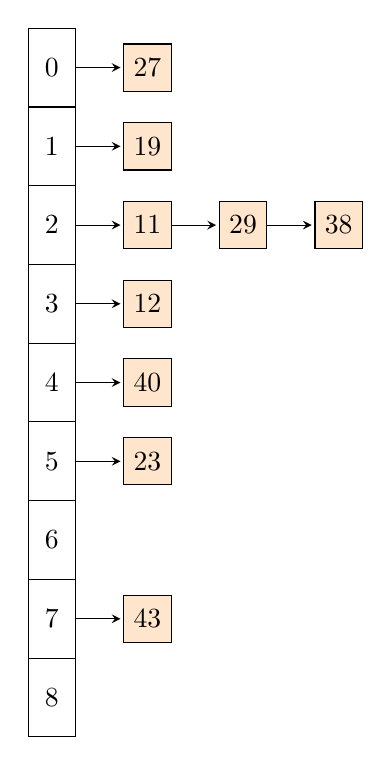
\begin{tikzpicture}
  \foreach \index/\list in {0/{27}, 1/{19}, 2/{11,29,38}, 3/{12}, 4/{40}, 5/{23}, 6/{}, 7/{43}, 8/{}} {
   \node[array element] (aux) at (0,-\index) {\index};
   \LinkedList{\list}
}
\end{tikzpicture}
\caption{Hash table with chaining}
\end{figure}
\end{minipage}

\newpage
\subsection*{Problem 7}
Consider inserting the keys 10, 23, 31, 4, 12, 28, 17, 87, 58 into a hash table of length $m=11$ using open addressing with the auxiliary hash function $h'(k)=k \Mod{m}$. Illustrate the result of inserting these keys using \textbf{linear probing}, using \textbf{quadratic probing} with $c_1=1$, and $c_2=3$, and using \textbf{double hashing} with $h_2(k)=1+(k \Mod{(m-1)})$. \\
% begin linear probing
\begin{minipage}{8cm}
\begin{align*}
  &\text{(1) insert}\ 10 \to 10 \Mod{11} = 10\\
  &\text{(2) insert}\ 23 \to 23 \Mod{11} = 1\\
  &\text{(3) insert}\ 31 \to 31 \Mod{11} = 9\\
  &\text{(4) insert}\ 4 \to 4 \Mod{11} = 4\\
  &\text{(5) insert}\ 12 \to  12 \Mod{11} = 1\ \times\text{collision} \\
  &\text{insert $12$ to slot $2$ because slot $1$ is occupied}&\\
  &\text{(6) insert}\ 28\to 28\Mod{11} = 6\\
  &\text{(7) insert}\ 17\to 17\Mod{11} = 6\ \times \\
  &\text{insert $17$ to index $7$ because slot $6$ is occupied}&\\
  &\text{(8) insert}\ 87\to 87\Mod{11} = 10\ \times \\
  &\text{insert $87$ to index $0$ because slot $10$ is occupied}&\\
  &\text{(9) insert}\ 58\to 58\Mod{11} = 3\\
\end{align*}
\end{minipage}
\qquad
\begin{minipage}{5cm}
\begin{figure}[H]
\centering
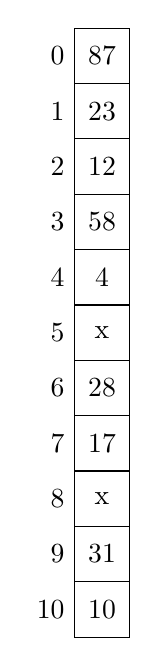
\begin{tikzpicture}
\coordinate (0);
\foreach \t[count=\i from 0,evaluate=\i as\j using int(\i+1)] in {
  87,
  23,
  12,
  58,
  4,
  x,
  28,
  17,
  x,
  31,
  10
}
\node at(\i.south)[anchor=north,draw,minimum height=2em,minimum width=2em,outer sep=0pt](\j){\t}
    node at(\j.west)[align=right,left]{\i}
    node at(\j.east)[align=left,right,xshift=-.7em]{};
\end{tikzpicture}
\caption{linear probing}
\end{figure}
\end{minipage}
% end linear probing
\par\noindent\rule{\textwidth}{0.4pt}
% start quadratic probing
\begin{minipage}{8cm}
\begin{align*}
  &\text{resolve collision:}\ h(k) + 1 * i + 3* i^2\Mod{11}\\
  &\text{(1) insert}\ 10 \to 10 \Mod{11} = 10\\
  &\text{(2) insert}\ 23 \to 23 \Mod{11} = 1\\
  &\text{(3) insert}\ 31 \to 31 \Mod{11} = 9\\
  &\text{(4) insert}\ 4 \to 4 \Mod{11} = 4\\
  &\text{(5) insert}\ 12 \to  12 \Mod{11} = 1\ \times\ \text{collision} \\
  &(1 + 1 + 3 * 1 * 1) \Mod{11} = (1 + 1 + 3) \Mod{11} = 5\\
  &\text{insert $12$ to slot $5$}\\
  &---------------------\\
  &\text{(6) insert}\ 28\to 28\Mod{11} = 6\\
  &\text{(7) insert}\ 17\to 17\Mod{11} = 6\ \times \\
  &(6 + 1 + 3 * 1 * 1) \Mod{11} = (6 + 1 + 3) \Mod{11} = 10\ \times \\
  &(6 + 2 + 3 * 2 * 2) \Mod{11} = (6 + 2 + 12) \Mod{11} = 9\ \times \\
  &(6 + 3 + 3 * 3 * 3) \Mod{11} = (6 + 3 + 27) \Mod{11} = 3 \\
  &\text{insert $17$ to slot $3$}\\
  &---------------------\\
  &\text{(8) insert}\ 87\to 87\Mod{11} = 10\ \times\\
  &(10 + 1 + 3 * 1 * 1) \mod{11} = (-1 + 1 + 3) \mod{11} = 3\ \times \\
  &(10 + 2 + 3 * 2 * 2) \mod{11} = (-1 + 2 + 12) \mod{11} = 2 \\
  &\text{insert $87$ to slot $2$}\\
  &---------------------\\
  &\text{(9) insert}\ 58\to 58\Mod{11} = 3\ \times\\
  &(3 + 1 + 3 * 1 * 1) \mod{11} = (3 + 1 + 3) \mod{11} = 7\\
  &\text{insert $58$ to slot $7$}\\
\end{align*}
\end{minipage}
\qquad
\begin{minipage}{5cm}
\begin{figure}[H]
\centering
% 7.2 quadratic hashing
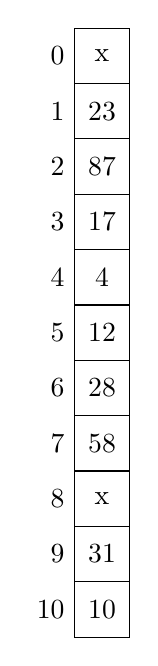
\begin{tikzpicture}
\coordinate (0);
\foreach \t[count=\i from 0,evaluate=\i as\j using int(\i+1)] in {
  x,
  23,
  87,
  17,
  4,
  12,
  28,
  58,
  x,
  31,
  10
}
\node at(\i.south)[anchor=north,draw,minimum height=2em,minimum width=2em,outer sep=0pt](\j){\t}
    node at(\j.west)[align=right,left]{\i}
    node at(\j.east)[align=left,right,xshift=-.7em]{};
\end{tikzpicture}
\caption{quadratic probing}
\end{figure}
\end{minipage}


% 7.3 double hashing
\begin{minipage}{8cm}
\begin{align*}
  &\text{resolve collision:}\ h_2(k) = 1 + k \Mod{10} \\
  & new_k = (h_1(k) + i * h_2(k)) \Mod{11}\\
  &\text{(1) insert}\ 10 \to 10 \Mod{11} = 10\\
  &\text{(2) insert}\ 23 \to 23 \Mod{11} = 1\\
  &\text{(3) insert}\ 31 \to 31 \Mod{11} = 9\\
  &\text{(4) insert}\ 4 \to 4 \Mod{11} = 4\\
  &\text{(5) insert}\ 12 \to  12 \Mod{11} = 1\ \times\text{collision} \\
  & h_2(12) = 1 + 12 \Mod{10} = 3\\
  & 1 + 1 * 3 \Mod{11} = 4\ \times \\
  & 1 + 2 * 3 \Mod{11} = 7\ \\
  &\text{insert $12$ to slot $7$}\\
  &---------------------\\
  &\text{(6) insert}\ 28\to 28\Mod{11} = 6\\
  &\text{(7) insert}\ 17\to 17\Mod{11} = 6\ \times \\
  & h_2(17) = 1 + 17 \Mod{10} = 8\\
  & 8 + 1 * 8 \Mod{11} = 5\\
  &\text{insert $17$ to slot $5$}\\
  &---------------------\\
  &\text{(8) insert}\ 87\to 87\Mod{11} = 10\ \times \\
  & h_2(87) = 1 + 87 \Mod{10} = 8\\
  & 8 + 1 * 8 \Mod{11} = 5\ \times \\
  & 8 + 2 * 8 \Mod{11} = 2\\
  &\text{insert $87$ to slot $2$}\\
  &---------------------\\
  &\text{(9) insert}\ 58\to 58\Mod{11} = 3\\
\end{align*}
\end{minipage}
\qquad
\begin{minipage}{5cm}
\begin{figure}[H]
\centering
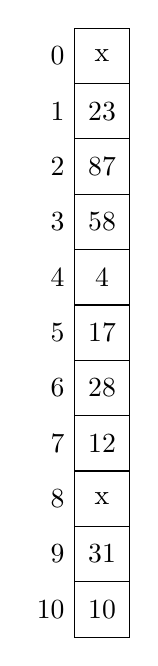
\begin{tikzpicture}
\coordinate (0);
\foreach \t[count=\i from 0,evaluate=\i as\j using int(\i+1)] in {
  x,
  23,
  87,
  58,
  4,
  17,
  28,
  12,
  x,
  31,
  10
}
\node at(\i.south)[anchor=north,draw,minimum height=2em,minimum width=2em,outer sep=0pt](\j){\t}
    node at(\j.west)[align=right,left]{\i}
    node at(\j.east)[align=left,right,xshift=-.7em]{};
\end{tikzpicture}
\caption{double hashing}
\end{figure}
\end{minipage}


\subsection*{Problem 8}
Solve the following assembly-line problem: \\ $e_1=1, e_2=1, x_1=7,x_2=3$ \\ $a_{1,1}=3, a_{1,2}=2,a_{1,3}=5, a_{1,4}=4, a_{1,5}=2$ \\ $a_{2,1}=4, a_{2,2}=2, a_{2,3}=4, a_{2,4}=6, a_{2,5}=4$ \\ $t_{1,1}=1, t_{1,2}=2, t_{1,3}=3, t_{1,4}=1$ \\ $t_{2,1}=2, t_{2,2}=3, t_{2,3}=1, t_{2,4}=2$.
\begin{figure}[H]
\centering
\begin{minipage}{5cm}
\centering
$\begin{NiceArray}{*{5}{c}}[first-row, first-col, last-col, hvlines]
\CodeBefore
\Body
       & 1 & 2 & 3 & 4 & 5 & \\
f_1[j] & 4 & 6 & 11 & 15 & 17 & 24\\
f_2[j] & 5 & 7 & 11 & 17 & 20 & 23
\end{NiceArray}$
\caption{f table}
\end{minipage}
\qquad
\begin{minipage}{5cm}
\centering
$\begin{NiceArray}{*{4}{c}}[first-row, first-col, hvlines]
\CodeBefore
\Body
       & 2 & 3 & 4 & 5 \\
l_1[j] & 1 & 1 & 1 & 1 \\
l_2[j] & 2 & 2 & 2 & 1
\end{NiceArray}$
\caption{l table}
\end{minipage}
\end{figure}

\begin{solution}
  $f^* = 23, l^* = 2$. The best solution for this assembly line is to start from $a_{1,1}$, and goes through $a_{1,2}, a_{1,3}, a_{1,4}, t_{1,4}, a_{2,5}, x_2$.
\end{solution}

\subsection*{Problem 9}
Find an optimal parenthesization of a matrix-chain product whose sequence of dimension is <5, 7, 3, 2, 4, 5>. \\
$A_1 = A_{5 \times 7}, A_2 = A_{7 \times 3}, A_3 = A_{3 \times 2}, A_4 = A_{2 \times 4}, A_5 = A_{4 \times 5}, p_0 = 5\label{p0}, p_1 = 7, p_2 = 3, p_3 = 2, p_4 = 4, p_5 = 5$\\
\begin{align*}
  m[1,2] &= 5 \cdot 7 \cdot 3 = 105\ (k = 1) \\
  m[2,3] &= 7 \cdot 3 \cdot 2 = 42\ (k = 2) \\
  m[3,4] &= 3 \cdot 2 \cdot 4 = 24\ (k = 3) \\
  m[4,5] &= 2 \cdot 4 \cdot 5 = 40\ (k = 4) \\
\end{align*}

\begin{align*}
  m[1,3] & =\left\{\begin{array}{cl}
      m[1,1] + m[2,3] + p_0\cdot p_1 \cdot p_3 &= 0 + 42 + 5 \cdot 7 \cdot 2 = 112\ (k = 1)\ \checkmark\\
      m[1,2] + m[3,3] + p_0\cdot p_2 \cdot p_3 &= 105 + 0 + 5 \cdot 3 \cdot 2 = 135 \\
  \end{array}\right. \\
  m[2,4] & =\left\{\begin{array}{cl}
      m[2,2] + m[3,4] + p_1\cdot p_2 \cdot p_4 &= 0 + 24 + 7 \cdot 3 \cdot 4 = 108\ \\
      m[2,3] + m[4,4] + p_1\cdot p_3 \cdot p_4 &= 42 + 0 + 7 \cdot 2 \cdot 4 = 98\ (k = 3)\ \checkmark\\
  \end{array}\right. \\
  m[3,5] & =\left\{\begin{array}{cl}
      m[3,3] + m[4,5] + p_2\cdot p_3 \cdot p_5 &= 0 + 40 + 3 \cdot 2 \cdot 5 = 70\ (k = 3)\ \checkmark\\
      m[3,4] + m[5,5] + p_2\cdot p_4 \cdot p_5 &= 24 + 0 + 3 \cdot 4 \cdot 5 = 84\\
  \end{array}\right. \\
  m[1,4] & =\left\{\begin{array}{cl}
      m[1,1] + m[2,4] + p_0\cdot p_1 \cdot p_4 &= 0 + 98 + 5 \cdot 7 \cdot 4 = 238 \\
      m[1,2] + m[3,4] + p_0\cdot p_2 \cdot p_4 &= 105 + 24 + 5 \cdot 3 \cdot 4 = 189\\
      m[1,3] + m[4,4] + p_0\cdot p_3 \cdot p_4 &= 112 + 0 + 5 \cdot 2 \cdot 4 = 152\ (k= 3)\checkmark\\
  \end{array}\right. \\
  m[2,5] & =\left\{\begin{array}{cl}
      m[2,2] + m[3,5] + p_1\cdot p_2 \cdot p_5 &= 0 + 70 + 7 \cdot 3 \cdot 5 = 175 \\
      m[2,3] + m[4,5] + p_1\cdot p_3 \cdot p_5 &= 42 + 40 + 7 \cdot 2 \cdot 5 = 152\ (k = 3)\checkmark\\
      m[2,4] + m[5,5] + p_1\cdot p_4 \cdot p_5 &= 98 + 0 + 7 \cdot 4 \cdot 5 = 238\\
  \end{array}\right. \\
  m[1,5] & =\left\{\begin{array}{cl}
      m[1,1] + m[2,5] + p_0\cdot p_1 \cdot p_5 &= 0 + 152 + 5\cdot 7 \cdot 5 = 327\\
      m[1,2] + m[3,5] + p_0\cdot p_2 \cdot p_5 &= 105 + 70 +5\cdot 3 \cdot 5 = 250\\
      m[1,3] + m[4,5] + p_0\cdot p_3 \cdot p_5 &= 112 + 40 +5\cdot 2 \cdot 5 = 202\ (k =3)\checkmark\\
      m[1,4] + m[5,5] + p_0\cdot p_4 \cdot p_5 &= 152 + 0 + 5\cdot 4 \cdot 5 = 252\\
  \end{array}\right. \\
\end{align*}

\begin{figure}[H]
\centering
\begin{minipage}{5cm}
\centering
\NiceMatrixOptions{cell-space-top-limit=1pt}
\begin{NiceTabular}{*{5}{c}}[first-row, first-col,corners=SE,hvlines, name=mtable]
\diagbox{j}{i}&1&2&3&4&5\\
5&202&152&70&40&0\\
4&152&98&24&0\\
3&112&42&0\\
2&105&0\\
1&0
\end{NiceTabular}
\caption{m table}
\end{minipage}
\qquad
\begin{minipage}{5cm}
\centering
\NiceMatrixOptions{cell-space-top-limit=1pt}
\begin{NiceTabular}{*{4}{c}}[first-row, first-col,corners=SE,hvlines, name=stable]
\diagbox{j}{i}&1&2&3&4\\
5&3&3&3&4\\
4&3&3&3\\
3&1&2\\
2&1\\
\end{NiceTabular}
\caption{s table}
\end{minipage}
\end{figure}

\begin{solution}
Positions of parenthesis: $((A_1(A_2A_3))(A_4A_5))\ or\ (((5 \times 7)((7 \times 3)(3 \times 2)))((2 \times 4)(4 \times 5)))$
\end{solution}

\subsection*{Problem 10}
Determine an LCS of <1, 1, 0, 1, 0, 1> and <0, 0, 1, 1, 0, 1, 1>.
\begin{solution}

\begin{figure}[H]
\centering
$\begin{NiceArray}{*{9}{c}}[first-row, first-col, hvlines, name=lcs]
\CodeBefore
\cellcolor{red!15}{1-5,1-6,1-7,1-8,1-9}
\cellcolor{red!15}{3-1,4-1,5-1,6-1,8-1}
\cellcolor{red!15}{8-9,7-8,6-8,5-7,4-6,3-5}
\Body
  & i & 0 & 1 & 2 & 3 & 4 & 5 & 6 & 7 \\
j &   & y_j & 0 & 0 & 1 & 1 & 0 & 1 & 1\\
0 & x_i & 0 & 0 & 0 & 0 & 0 & 0 & 0 & 0\\
1 & 1   & 0 & \thead{\uparrow \\0} & \thead{\uparrow \\0} & \thead{\nwarrow \\1} & \thead{\nwarrow \\1} & \thead{\leftarrow \\1} & \thead{\nwarrow \\1} & \thead{\nwarrow \\1}\\
2 & 1   & 0 & \thead{\uparrow \\0} & \thead{\uparrow \\0} & \thead{\nwarrow \\1} & \thead{\nwarrow \\2} & \thead{\leftarrow \\2} & \thead{\nwarrow \\2} & \thead{\nwarrow \\2}\\
3 & 0   & 0 & \thead{\nwarrow \\1} & \thead{\nwarrow \\1} & \thead{\leftarrow \\1} & \thead{\uparrow \\2} & \thead{\nwarrow \\3} & \thead{\leftarrow \\3} & \thead{\leftarrow \\3}\\
4 & 1   & 0 & \thead{\uparrow \\1} & \thead{\uparrow \\1} & \thead{\nwarrow \\2} & \thead{\nwarrow \\2} & \thead{\uparrow \\3} & \thead{\nwarrow \\4} & \thead{\nwarrow \\4}\\
5 & 0   & 0 & \thead{\nwarrow \\1} & \thead{\nwarrow \\2} & \thead{\uparrow \\2} & \thead{\uparrow \\2} & \thead{\nwarrow \\3} & \thead{\uparrow \\4} & \thead{\uparrow \\4}\\
6 & 1   & 0 & \thead{\uparrow \\1} & \thead{\uparrow \\2} & \thead{\nwarrow \\3} & \thead{\nwarrow \\3} & \thead{\uparrow \\3} & \thead{\nwarrow \\4} & \thead{\nwarrow \\5}\\
\CodeAfter
  \tikz \draw (lcs-1-5) circle (2mm) ;
  \tikz \draw (lcs-1-6) circle (2mm) ;
  \tikz \draw (lcs-1-7) circle (2mm) ;
  \tikz \draw (lcs-1-8) circle (2mm) ;
  \tikz \draw (lcs-1-9) circle (2mm) ;
  \tikz \draw (lcs-3-1) circle (2mm) ;
  \tikz \draw (lcs-4-1) circle (2mm) ;
  \tikz \draw (lcs-5-1) circle (2mm) ;
  \tikz \draw (lcs-6-1) circle (2mm) ;
  \tikz \draw (lcs-8-1) circle (2mm) ;
  \tikz \draw (lcs-8-9) circle (3.5mm) ;
  \tikz \draw (lcs-7-8) circle (3.5mm) ;
  \tikz \draw (lcs-6-8) circle (3.5mm) ;
  \tikz \draw (lcs-5-7) circle (3.5mm) ;
  \tikz \draw (lcs-4-6) circle (3.5mm) ;
  \tikz \draw (lcs-3-5) circle (3.5mm) ;
\end{NiceArray}$
\caption{c table for LCS}
\end{figure}

Thus, the longest common sequence is < 1, 1, 0, 1, 1>.
\end{solution}

\end{document}


